% Created 2021-06-07 Mon 18:42
% Intended LaTeX compiler: pdflatex
\documentclass[presentation]{beamer}
\usepackage[utf8]{inputenc}
\usepackage[T1]{fontenc}
\usepackage{graphicx}
\usepackage{grffile}
\usepackage{longtable}
\usepackage{wrapfig}
\usepackage{rotating}
\usepackage[normalem]{ulem}
\usepackage{amsmath}
\usepackage{textcomp}
\usepackage{amssymb}
\usepackage{capt-of}
\usepackage{hyperref}
\usepackage{minted}
\usemintedstyle{trac}
\setminted{fontsize=\scriptsize,baselinestretch=1}
\author{Igor Dejanović}
\date{\today}
\title{Pharo\\\medskip
\large Bazirano na \href{http://mooc.pharo.org}{Pharo MOOC}}
\hypersetup{
 pdfauthor={Igor Dejanović},
 pdftitle={Pharo},
 pdfkeywords={},
 pdfsubject={},
 pdfcreator={Emacs 27.2 (Org mode 9.4.5)}, 
 pdflang={English}}
\begin{document}

\maketitle

\section{Smalltalk}
\label{sec:orgb429961}
\subsection{Šta je Smalltalk?}
\label{sec:org78e2acd}
\begin{itemize}
\item Objektno-orijentisani dinamički reflektivni jezik.
\item Xerox PARC - Alan Kay, Dan Ingalls i drugi - tokom 70-ih.
\item Uticao na razvoj Actor model obrasca.
\item Nastao pod uticajem Simule (prvi OO jezik, Norwegian Computing Center u Oslu -
60-te).
\item Jedan od najuticajnijih jezika.
\item Napredni koncepti: sve je objekat, razmena poruka, ``živ'' sistem, virtualna
mašina.
\item Konstrukcionistički pristup programiranju.
\end{itemize}

\begin{itemize}
\item \url{https://en.wikipedia.org/wiki/PARC\_(company)}
\item \url{https://en.wikipedia.org/wiki/Smalltalk}
\end{itemize}

\subsection{Istorijat}
\label{sec:orge0fb4ae}
\begin{itemize}
\item Razvijen u par dana 1971 godine (\emph{Smalltalk-71}) zbog opklade (Alan Kay).
\item Kasnija verzija \emph{Smalltalk-72} je korišćena u istraživanjima.
\item \emph{Smalltalk-76} - nasleđivanje klasa, razvojno okruženje
\item Najpoznatija verzija Smalltalk-80 - meta-klase. Prva verzija dostupna van
PARC-a (Apple, HP, DEC, UC Berkeley)
\item Standardizovan - ANSI 1998
\end{itemize}
\subsection{Smalltalk implementacije}
\label{sec:org67067ac}
\begin{itemize}
\item Komercijalne
\begin{itemize}
\item \emph{Smalltalk-80} (Xerox PARC)
\item \emph{VisualWorks} (ParcPlace Systems, prodato 1999 firmi Cincom)
\item \emph{IBM VisualAge} - napušteno u korist Jave. Današnji Eclipse je započeo kao
VisualAge Smalltalk okruženje. Jedno vreme je i Java podrška bila
implementirana u Smalltalk-u.
\end{itemize}

\item FLOSS:
\begin{itemize}
\item Squeak (moderna verzija Smalltalk-80) - Apple -> Disney -> HP Labs -> SAP
Labs -> Y Combinator
\item Pharo - fork Squeak-a (2008) sa ciljem upotrebe u istraživanju i
komercijalnim projektima (Pharo consortium, Pharo association)
\item Amber Smalltalk - Smalltalk u JavaScrript-u
\end{itemize}
\end{itemize}

\begin{itemize}
\item \url{https://en.wikipedia.org/wiki/VisualAge}
\item \url{https://en.wikipedia.org/wiki/Squeak}
\end{itemize}

\subsection{Familija Smalltalk i vezanih jezika}
\label{sec:orgb5f059e}

\begin{center}
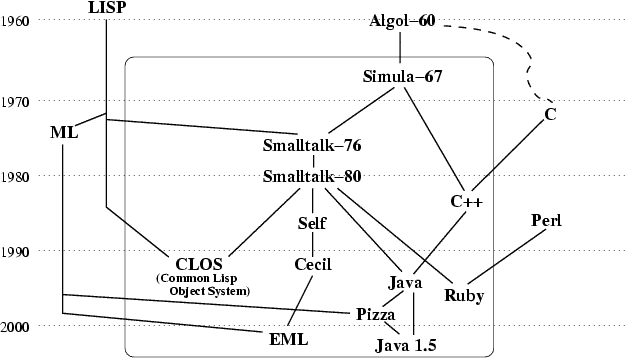
\includegraphics[width=.9\linewidth]{./slike/smalltalk-history.png}
\end{center}

\url{http://courses.cs.washington.edu/courses/cse341/04wi/lectures/16-smalltalk-intro.html}

\section{Pharo uvod}
\label{sec:org382525c}
\subsection{Pharo}
\label{sec:orga0c09f7}

\begin{itemize}
\item Pravi OO jezik (``sve je objekat'') + IDE!
\item Inspirisan Smalltalk-om
\item Aktivna zajednica
\item ``Živ'' sistem.
\item Jednostavan i moćan objektni model
\item Radi na Mac OSX, Linux, iOS, Android, Windows, Pi.
\item 100\% MIT
\item \href{https://github.com/pavel-krivanek/pharoMaterials/blob/master/features/PharoKeyFeatures.md}{Pregled nekih osobina Pharo IDE i jezika}
\end{itemize}

\subsection{Pharo instalacija}
\label{sec:orge29b852}

\begin{itemize}
\item Preporučena upotreba \href{https://pharo.org/download}{Pharo Launcher} alata
\begin{itemize}
\item Instalacija i upravljanje slikama i virtualnim mašinama
\end{itemize}

\item Alternativno, može se koristiti \href{http://get.pharo.org/}{Zeroconf skripta}:
\end{itemize}

\begin{verbatim}
# 64bit version
mkdir pharo
cd pharo
curl -L https://get.pharo.org/64/ | bash
# or if curl is not available:
wget -O- https://get.pharo.org/64 | bash
\end{verbatim}

\begin{verbatim}
# 32bit version
curl -L https://get.pharo.org | bash
# or if curl is not available:
wget -O- https://get.pharo.org | bash
\end{verbatim}

\subsection{Pharo fajl komponente}
\label{sec:org17fc3e4}

\begin{verbatim}
pharo
Pharo8.0-32bit-a153e04
Pharo.changes
Pharo.image
pharo-ui
pharo-vm
\end{verbatim}

\begin{itemize}
\item \texttt{pharo-vm} - Pharo virtuelna mašina (\emph{OS-specific})
\item \texttt{Pharo.image} - Perzistirano stanje/objekti
\item \texttt{Pharo...sources} - Izvorni kod izdanja
\item \texttt{Pharo.changes} - Promene u izvornom kodu od početka upotrebe
\end{itemize}

\begin{itemize}
\item \texttt{Pharo.image} i \texttt{Pharo.changes} su fajlovi gde dolazi do promena
\item \texttt{Pharo.changes} se menja kada menjamo kod
\item \texttt{Pharo.image} se menja kada eksplicitno tražimo perzistenciju stanja
\end{itemize}

\subsection{Cela sintaksa}
\label{sec:org16e84c1}

Staje na jedan slajd:

\begin{verbatim}
exampleWithNumber: x
    "A method that illustrates every part of Smalltalk method syntax."
    <menu>
    | y |
    true & false not & (nil isNil) ifFalse: [self halt].
    y := self size + super size.
    #($a #a "a" 1 1.0)
        do: [ :each |
            Transcript show: (each class name);
                       show: (each printString);
                       show: ' '].
    ^x < y
\end{verbatim}

\subsection{Model}
\label{sec:org235338b}

\begin{itemize}
\item Dinamički tipiziran
\item Sve je objekat tj. instanca klase
\item Sve metode su javne i virtualne
\item Svi atributi su zaštićeni
\item Jednostruko nasleđivanje (\emph{Single inheritance})
\end{itemize}

\subsection{Napisan u samom sebi}
\label{sec:org9e924a8}

\begin{itemize}
\item Sve je napisano u Pharo!
\item Jednostavna sintaksa/model za pristup svemu.

\begin{center}

\includegraphics[width=.9\linewidth]{./slike/hands.jpg}
\end{center}
\end{itemize}

\subsection{Introspekcija}
\label{sec:orgb48ab58}

\begin{itemize}
\item Pharo nije ``crna kutija''.
\item Sve što vidite su objekti sa kojima možete stupiti u interakciju i menjati ih
``naživo''.
\item Program koji se razvija je nerazdvojni deo razvojnog okruženja.
\item Npr. \texttt{Alt+Shift+Click} -> Halo hendleri!
\end{itemize}

\begin{center}
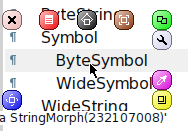
\includegraphics[width=.9\linewidth]{./slike/halo.png}
\end{center}

\subsection{Samo objekti, poruke\ldots{}}
\label{sec:orgbfeb4ad}

\begin{itemize}
\item \emph{Objekti}: mouse pointer, booleans, arrays, numbers, strings, windows, files,
sound, url, socket, font, text, streams\ldots{}
\item \emph{Poruke (messages)}: \texttt{size}, \texttt{+}, \texttt{at:put:}, \texttt{do:}, \texttt{collect:},
\texttt{ifTrue:ifFalse:}\ldots{}
\item Poruke predstavljaju \textbf{\textbf{nameru}} (šta treba uraditi). Metode opisuju kako treba
nešto uraditi.
\item Objekat koji prima poruku zovemo \textbf{\textbf{prijemnikom}} (\emph{receiver}).
\end{itemize}

\subsection{\ldots{} i blokovi (\emph{Block Closures})}
\label{sec:orge90eb0c}

\begin{itemize}
\item Blokovi su vrsta anonimnih metoda.
\end{itemize}

\begin{verbatim}
4 timesRepeat:
    [ Transcript show: 'Hello World!']
\end{verbatim}

\begin{itemize}
\item Blokovi se navode unutar \texttt{[]}.
\end{itemize}

\subsection{Jednostavan, elegantan i uniforman model}
\label{sec:org8257906}

\begin{itemize}
\item \emph{Sve} je objekat tj. instanca klase.
\begin{itemize}
\item Klase i poruke su takođe objekti.
\end{itemize}
\item Svo procesiranje se obavlja \textbf{\textbf{razmenom poruka}} (\emph{message passing}) između
objekata.

\item Koristimo izraz \textbf{\textbf{slanje poruke}} jer:
\begin{itemize}
\item metode se određuju dinamički
\item \textbf{\textbf{kasno povezivanje}} (\emph{late binding}), samo virtuelni pozivi
\end{itemize}

\item Postoji \textbf{\textbf{samo jedan}} mehanizam za pretragu metoda za sve objekte.
\end{itemize}

\subsection{Pharo objektni model}
\label{sec:org9484f8d}

\begin{itemize}
\item Atributi instanci (\emph{instance variables}) su zaštićeni (\emph{protected}):
\begin{itemize}
\item Privatni za objekat
\item Dostupni podklasama
\end{itemize}
\item Metode su javne (\emph{public}) i virtualne.
\item Jednostruko nasleđivanje klasa.
\end{itemize}

\subsection{Slanje poruka}
\label{sec:orgd65163f}

\begin{verbatim}
Date today

Date today + 3 days

2 + 3

(point1 x * point2 y) - (point1 y * point2 x)
\end{verbatim}

\subsection{Kreiranje objekata}
\label{sec:org004bb57}

Obavlja se slanjem poruke drugom objektu

\begin{verbatim}
10@20
\end{verbatim}

Nova instanca klase \texttt{Point} se kreira:

\begin{itemize}
\item slanjem poruke \texttt{@}
\item objektu \texttt{10} (\texttt{SmallInteger})
\item sa argumentom \texttt{20} (\texttt{SmallInteger})
\end{itemize}

\subsection{Kreiranje objekata - String}
\label{sec:org677fcff}

\begin{verbatim}
'Pharo', 'is cool!'
=> 'Pharo is cool!'
\end{verbatim}

Novi string se kreira spajanjem dva stringa tako što:
\begin{itemize}
\item se šalje poruka \texttt{,}
\item stringu \texttt{'Pharo'}
\item sa parametrom \texttt{'is cool!'}
\end{itemize}

\subsection{Kreiranje objekata}
\label{sec:orgfb00acb}

Slanjem poruke \texttt{new} ili \texttt{new:} klasi

\begin{verbatim}
Monster new
=> aMonster
\end{verbatim}

U prethodnom primeru \texttt{Monster} je ime klase a \texttt{new} je poruka koja se šalje ovoj
klasi. Rezultat je nova instanca klase \texttt{Monster}.

Kreiranje niza dužine 6.

\begin{verbatim}
Array new: 6
=> #(nil nil nil nil nil nil)
\end{verbatim}

Slanjem poruke klasi izvšava se metoda klase (\emph{class method}).

\begin{verbatim}
Tamagoshi withHunger: 10
\end{verbatim}

\subsection{Less is more!}
\label{sec:org1b5941b}

\begin{itemize}
\item Bez konstruktora
\item Bez statičkih metoda
\item Bez deklaracije tipova
\item Bez interfejsa
\item Bez \emph{package/private/protected} modifikatora
\item Bez parametrizovanih tipova
\item Bez boxing-a
\item Ali i dalje vrlo moćan jezik!
\end{itemize}

\subsection{Hello world}
\label{sec:org99cc0d2}

\begin{verbatim}
'Hello World' asMorph openInWindow
\end{verbatim}

Šaljemo poruku \texttt{asMorph} stringu \texttt{Hello World} i dobijamo grafički element
(\emph{Morph}). Dobijenom grafičkom elementu šaljemo poruku \texttt{openInWindow} da bi ga
prikazali u prozoru.

\subsection{Primer - preuzimanje slike sa web-a}
\label{sec:org9fbc6d6}

\begin{verbatim}
(ZnEasy getPng: 'http://pharo.org/web/files/pharo.png') asMorph openInWindow
\end{verbatim}

\begin{itemize}
\item \texttt{ZnEasy} je ime klase. Klase su globalno dostupe i nazivi počinju sa velikim
slovom.
\item \texttt{getPng:} je poruka koju šaljemo klasi \texttt{ZnEasy}. Ova poruka ima argument. U
ovom slučaju to je string \texttt{'http://pharo.org/web/files/pharo.png'}
\begin{itemize}
\item Poruke koje imaju argumente se pišu sa \texttt{:} na kraju naziva i mogu biti
višesložne. Ovakve poruke nazivamo \texttt{keyword message}.
\end{itemize}

\item Poruka \texttt{asMorph} šalje se objektu koji vraća poruka \texttt{getPng:}. Ovo je obična
unarna poruka bez argumenata.

\item Poruka \texttt{openInWindow} se šalje objektu koji vraća poruka \texttt{asMorph}.

\item Ove dve unarne poruke se primenjuju s leva na desno.
\end{itemize}

\subsection{Sintaksni elementi jezika}
\label{sec:orge2a902e}

\begin{center}
\begin{tabular}{ll}
Vrsta & Primer\\
\hline
Komentar & \texttt{"Ovo je komentar"}\\
Karakteri & \texttt{\$c} \texttt{\$\#} \texttt{\$@}\\
String & \texttt{'Ovo je string'}\\
Simbol (jedinstveni string) & \texttt{\#prvi} \texttt{\#+}\\
Literal niz & \texttt{\#(23 56 89)}\\
Integer & \texttt{45}, \texttt{2r10100}\\
Real & \texttt{1.5}, \texttt{6.03e-34}, \texttt{4}, \texttt{2.4e7}\\
\end{tabular}
\end{center}

\subsection{Sintaksni elementi jezika}
\label{sec:org159d97a}

\begin{center}
\begin{tabular}{ll}
Vrsta & Primer\\
\hline
Boolean & \texttt{true}, \texttt{false}\\
 & (instanca \texttt{True} i \texttt{False})\\
Undefined & \texttt{nil} (instanca \texttt{UndefinedObject} )\\
Point & \texttt{10@120}\\
\end{tabular}
\end{center}

\subsection{Osnovne jezičke konstrukcije}
\label{sec:orga8eb8b9}

\begin{itemize}
\item Deklaracija privremene varijable: \texttt{| var |}
\item Dodela vrednosti varijabli: \texttt{var := aValue}
\item Separator iskaza: \texttt{obj1 message1. obj2 message2.}
\item Povratak vrednosti iz metode: \texttt{\textasciicircum{} aValue}
\item Blokovi (leksička zatvorenja ili anonimne metode)
\end{itemize}

\begin{verbatim}
[ :x | x + 2 ] value: 5
=> 7
\end{verbatim}

\section{Poruke}
\label{sec:org2d0a022}
\subsection{Tri vrste poruka}
\label{sec:orgc9c382e}

\begin{enumerate}
\item Unarne poruke:
\begin{itemize}
\item Sintaksa: \texttt{receiver selector}
\item Primeri:
\end{itemize}
\begin{verbatim}
   9 squared
   Date today
\end{verbatim}

\item Binarne poruke:
\begin{itemize}
\item Sintaksa: \texttt{receiver selector argument}
\item Primeri:
\end{itemize}
\begin{verbatim}
   2 + 3
   3 @ 4
\end{verbatim}

\item \emph{Keyword} poruke:
\begin{itemize}
\item Sintaksa: \texttt{receiver key1: arg1 key2: arg2}
\item Primeri:
\end{itemize}
\begin{verbatim}
   2 between: 10 and: 20
   5 to: 10 do: [ :i | Transcript show: i ]
\end{verbatim}
\end{enumerate}

\subsection{Slanje unarne poruke}
\label{sec:org4adc49a}

\begin{verbatim}
receiver selector
\end{verbatim}

Primer:

\begin{verbatim}
10000 factorial
\end{verbatim}


Šaljemo poruku \texttt{factorial} objektu \texttt{10000}.

\subsection{Slanje binarne poruke}
\label{sec:org60b66d3}

\begin{verbatim}
receiver selector argument
\end{verbatim}

Primer:

\begin{verbatim}
1 + 3
\end{verbatim}

Šaljemo poruku \texttt{+} objektu \texttt{1} sa parametrom \texttt{3}.

\subsection{Slanje \emph{keyword} poruke}
\label{sec:orgfdbcb87}

\begin{verbatim}
receiver keyword1: arg1 keyword2: arg2
\end{verbatim}

Ekvivalentno u Javi ili C-like jezicima:

\begin{verbatim}
receiver.keyword1keyword2(arg1, arg2)
\end{verbatim}

\subsection{\emph{Keyword} poruke za Java programere}
\label{sec:org71cee49}

U Javi

\begin{verbatim}
postman.send(mail, recipient);
\end{verbatim}

\begin{verbatim}
postman . send ( mail , recipient );
\end{verbatim}

\begin{verbatim}
postman send mail recipient
\end{verbatim}

\begin{verbatim}
postman send mail to recipient
\end{verbatim}

U Pharo/Smalltalk-u

\begin{verbatim}
postman send: mail to: recipient
\end{verbatim}

\subsection{Primer: slanje HTTP zahteva}
\label{sec:org9e3f1f1}

\begin{verbatim}
ZnClient new
  url: 'https://en.wikipedia.org/w/index.php';
  queryAt:'title' put:'Pharo';
  queryAt:'action' put:'edit';
  get
\end{verbatim}

\begin{itemize}
\item \texttt{new} je unarna poruka koja se šalje klasi \texttt{ZnClient}
\item \texttt{queryAt:put:} je \emph{keyword} poruka sa dva argumenta
\item \texttt{get} je unarna poruka
\item \texttt{;} je specijalan operator koji zovemo kaskada (\emph{cascade}) - šaljemo poruku
istom objektu primaocu.
\end{itemize}

\subsection{Poruke su svuda}
\label{sec:orga16d4de}

\begin{itemize}
\item Uslovi
\item Petlje
\item Iteracije
\item Konkurencija
\item \ldots{}
\end{itemize}

\subsection{Primer - \texttt{Integer>>factorial}}
\label{sec:org305d836}

\begin{verbatim}
factorial
	"Answer the factorial of the receiver."

	self = 0 ifTrue: [^ 1].
	self > 0 ifTrue: [^ self * (self - 1) factorial].
	self error: 'Not valid for negative integers'
\end{verbatim}

\begin{itemize}
\item \texttt{ifTrue:} je poruka koja se šalje \texttt{Boolean} objektu koji vraća poruka \texttt{=}
poslata objektu \texttt{self} sa parametrom \texttt{0}.
\item Postoje i \texttt{ifTrue:ifFalse:}, \texttt{ifFalse:ifTrue:} i \texttt{ifFalse:}
\item Implementirane su u klasama \texttt{True} i \texttt{False} i možete ih pročitati. Ne postoji
ništa specijalno u vezi ovih poruka!
\end{itemize}

\subsection{Kompozicija poruka - s leva na desno}
\label{sec:org4be6691}

Šta se dešava kada imamo sukcesivne poruke istog tipa?

\begin{verbatim}
1000 factorial class name
> 'LargePositiveInteger'
\end{verbatim}

ekvivalentno je sa:

\begin{verbatim}
(((1000 factorial) class) name)
\end{verbatim}

\subsection{Prioriteti poruka}
\label{sec:org8a895ed}

\begin{verbatim}
(Msg) > Unary > Binary > Keywords
\end{verbatim}

Ova pravila redukuju potrebu za navođenjem zagrada.

\subsection{Prioritet primeri}
\label{sec:orgf780930}

\begin{verbatim}
2 + 3 squared
> 2 + 9
> 11
\end{verbatim}

\begin{itemize}
\item Prvo unarna \texttt{squared}
\item Zatim binarna \texttt{+}
\end{itemize}

\subsection{Prioritet primeri}
\label{sec:org9487480}

\begin{verbatim}
2 raisedTo: 3 + 2
> 2 raisedTo: 5
> 32
\end{verbatim}

\begin{itemize}
\item Prvo binarna \texttt{+}
\item Zatim \emph{keyword} \texttt{raisedTo:}
\end{itemize}

\subsection{Prioritet primeri}
\label{sec:org701372b}

\begin{verbatim}
Color gray - Color white = Color black
> aGray - aWhite = aBlack
> aBlack = aBlack
> true
\end{verbatim}

\begin{itemize}
\item Prvo unarne
\item Zatim binarne s leva na desno: \texttt{-} pa onda \texttt{=}
\end{itemize}

\subsection{Prioritet primeri}
\label{sec:org172aa31}

\begin{verbatim}
1 class maxVal + 1
> 1073741824
\end{verbatim}

\begin{itemize}
\item unarna \texttt{class}, unarna \texttt{maxVal}, binarna \texttt{+}
\end{itemize}

\begin{verbatim}
1 class
> SmallInteger

1 class maxVal
> 1073741823

1 class maxVal + 1
> 1073741824

(1 class maxVal + 1) class
> LargePositiveInteger
\end{verbatim}

\subsection{Upotreba zagrada kod prioriteta}
\label{sec:org9640650}

\begin{verbatim}
0@0 extent: 100@100 bottomRight
> Message not understood
> 100 does not understand bottomRight
\end{verbatim}

Moramo koristiti zagrade:

\begin{verbatim}
(0@0 extent: 100@100) bottomRight
> (aPoint extent: anotherPoint) bottomRight
> aRectangle bottomRight
> 100@100
\end{verbatim}

\subsection{Cena jednostavnosti/uniformnosti}
\label{sec:orgb837395}

Samo poruke:

\begin{itemize}
\item \texttt{+}
\begin{itemize}
\item je poruka (nije operacija), ne postoji specijalno definisani prioritet
\item možemo je redefinisati za različite domene
\end{itemize}
\item Jednostavnost
\item Ograničenje: nemamo definisan matematički prioritet operacija
\end{itemize}

\subsection{Nema prioriteta aritmetičkih operacija}
\label{sec:org690c39b}

\begin{verbatim}
3 + 2 * 10
> 5 * 10
> 50
\end{verbatim}

Moramo pisati sa zagradama:

\begin{verbatim}
3 + (2 * 10)
> 3 + 20
> 23
\end{verbatim}

\subsection{Nema prioriteta aritmetičkih operacija}
\label{sec:org42c5dd6}

\begin{verbatim}
1/3 + 2/3
> 7/3 /3
> 7/9
\end{verbatim}

Moramo pisati:

\begin{verbatim}
(1/3) + (2/3)
>1
\end{verbatim}

\subsection{Sekvenca izraza}
\label{sec:org6fab431}

\texttt{.} je separator:

\begin{verbatim}
expression1.
expression2.
expression3
\end{verbatim}

Primer:

\begin{verbatim}
Transcript cr.
Transcript show: 1.
Transcript show: 2
\end{verbatim}

\subsection{Sekvenca izraza}
\label{sec:orga467273}

\begin{itemize}
\item \texttt{.} je separator a ne terminacija.
\item Nema potrebe da se stavlja na kraju niza izraza.
\item Ne stavlja se posle deklaracije privremenih promenjivih.
\end{itemize}

\begin{verbatim}
| macNode pcNode |
macNode := Workstation withName: #mac.
macNode sendPacket: 'Hello World'
\end{verbatim}

\subsection{Slanje više poruka istom objektu - kaskada (\texttt{;})}
\label{sec:orgdac85cc}

\begin{verbatim}
|c|
c := OrderedCollection new.
c add: 1.
c add: 2
\end{verbatim}

Ekvivalentno je sa:

\begin{verbatim}
OrderedCollection new
   add: 1;
   add: 2
\end{verbatim}

\begin{itemize}
\item \texttt{add: 2} se šalje istom prijemniku poruke \texttt{add: 1} a to je objekat vraćen
porukom \texttt{new}.
\end{itemize}

\section{Blokovi}
\label{sec:orgcbb58b0}
\subsection{Blokovi izgledaju kao funkcije}
\label{sec:orgeb3fabb}


fct(x) = x*x + 3

\begin{verbatim}
fct := [ :x | x * x + 3 ]
\end{verbatim}

fct(2)

\begin{verbatim}
fct value: 2
\end{verbatim}

\subsection{Blokovi}
\label{sec:org7cee539}

\begin{itemize}
\item Anonimne metode
\end{itemize}

\begin{verbatim}
[ :each | Transcript show: each abs printString; cr ]
\end{verbatim}

\begin{itemize}
\item Leksička ``zatvorenja'' (\emph{closures})
\item Takođe su objekti:
\begin{itemize}
\item Mogu se proslediti kao argumenti poruka
\item Mogu se dodeliti varijablama
\item Mogu biti povratne vrednosti metoda
\end{itemize}
\end{itemize}

\subsection{Upotreba blokova}
\label{sec:orgccab48a}

\begin{verbatim}
#(1 2 -4 -86) do: [ :each | Transcript show: each abs printString; cr ]
> 1
> 2
> 4
> 86
\end{verbatim}

\begin{itemize}
\item Pišu se unutar \texttt{[]}
\item Mogu imati parametre - navode se kao simboli pre \texttt{|} (\texttt{:each})
\item U ovom primeru blok se evaluira za svaki element niza. \texttt{:each} dobija redom
vrednosti niza.
\item \texttt{value:} poruka se koristi za evaluaciju bloka.
\end{itemize}

\subsection{Definicija bloka ne izvršava kod}
\label{sec:org02a9183}

\begin{verbatim}
(1/0)
-> Greška
\end{verbatim}

Ali nema greške pri definiciji bloka:
\begin{itemize}
\item Definicija bloka ne izvršava kod
\item Definicija bloka ``zamrzava'' izračunavanje definisano telom bloka.
\end{itemize}

\begin{verbatim}
[1/0]
> [1/0]

[1/0].
1 + 2
> 3
\end{verbatim}

\subsection{Izvršavanje blokova}
\label{sec:org979eded}

Obavlja se eksplicitno slanjem poruke \texttt{value}.

\begin{verbatim}
[2 + 6] value
> 8

[1/0] value
> Error
\end{verbatim}

\subsection{Blok sa jednim argumentom}
\label{sec:orgb38b62e}

Blokovi mogu imati argumente (kao i metode):

\begin{verbatim}
[ :x | x + 2 ]
\end{verbatim}

\begin{itemize}
\item \texttt{:x} predstavlja argument bloka
\item \texttt{x + 2} je telo bloka
\end{itemize}

\begin{verbatim}
[ :x | x + 2 ] value: 5
> 7
\end{verbatim}

\begin{itemize}
\item Poruka \texttt{value:} izvršava blok sa parametrom \texttt{5}.
\begin{itemize}
\item \texttt{x} dobija vrednost \texttt{5} za vreme izvršavanja bloka.
\end{itemize}
\end{itemize}

\subsection{Vrednost evaluacije bloka}
\label{sec:org5d1d189}

Evaluacija bloka vraća vrednost poslednjeg izraza u bloku:

\begin{verbatim}
[:x|
 x + 33.
 x + 2] value: 5
> 7
\end{verbatim}

\subsection{Blokovi se mogu sačuvati}
\label{sec:org6f423a8}

\begin{itemize}
\item Blok se može sačuvati kao vrednost varijable
\item Blok se može evaluirati više puta
\end{itemize}

\begin{verbatim}
| add2 |
add2 := [ :x | x + 2 ].
add2 value: 5.
>7

add2 value: 33
> 35
\end{verbatim}

\subsection{Blokovi mogu imati više argumenata}
\label{sec:orge13ad27}

Primer:

\begin{verbatim}
[ :x :y | x + y ]
\end{verbatim}

\texttt{:x :y} su argumenti bloka.

Kako se izvršava blok sa dva argumenta?

\begin{verbatim}
[ :x :y | x + y ] ??? 5 7
> 12
\end{verbatim}

\begin{verbatim}
[ :x :y | x + y ] value: 5 value: 7
> 12
\end{verbatim}

\begin{itemize}
\item \texttt{value:value:} je poruka sa dva argumenta koja se šalje bloku sa parametrima
\texttt{5} i \texttt{7}
\end{itemize}

\subsection{Blokovi sa privremenim varijablama}
\label{sec:org9cc0863}

Blokovi mogu definisati lokalne privremene varijable (kao i metode):

\begin{verbatim}
Collection>>affect: anObject when: aBoolean
  self do: [ :index | | args |
            args := ....
            aBoolean
            ifTrue: [ anObject do: args ]
            ifFalse: [ anObject doDifferently: args ] ].

\end{verbatim}

\begin{itemize}
\item \texttt{| args |} definiše privremenu varijablu \texttt{args}
\item \texttt{args} postoji samo za vreme izvršavanja bloka
\end{itemize}

\subsection{Povratak iz bloka izaziva povratak iz metode}
\label{sec:orgb5f63f3}

Kada se \texttt{\textasciicircum{}} izvrši unutar bloka dolazi do povratka iz metode u kojoj je blok
definisan:

\begin{verbatim}
Integer>>factorial
  "Answer the factorial of the receiver."

  self = 0 ifTrue: [ ^ 1 ].
  self > 0 ifTrue: [ ^ self * (self − 1) factorial ].
  self error: 'Not valid for negative integers'
\end{verbatim}

\begin{verbatim}
0 factorial
>1

42 factorial
>1405006117752879898543142606244511569936384000000000
\end{verbatim}

\subsection{Dizajn saveti za upotrebu blokova}
\label{sec:org43d7f8a}

\begin{itemize}
\item Koristi blokove sa najviše 2 ili 3 parametra
\item Definisati klasu umesto bloka za više parametara
\end{itemize}

\section{Petlje i iteracije}
\label{sec:orgf9e706e}
\subsection{Petlje su takođe implementirane kao poruke}
\label{sec:org4439f95}

\begin{verbatim}
1 to: 4 do: [ :i | Transcript << i ]
> 1
> 2
> 3
> 4
\end{verbatim}

\begin{itemize}
\item \texttt{to:do:} je poruka poslata broju (instanci \texttt{Integer} klase)
\end{itemize}

\subsection{Petlje su takođe implementirane kao poruke}
\label{sec:org3160ce4}

\begin{itemize}
\item Mnoge druge vrste petlji: \texttt{timesRepeat:}, \texttt{to:by:do:}, \texttt{whileTrue:},
\texttt{whileFalse:}\ldots{}
\end{itemize}

\begin{verbatim}
4 timesRepeat: [self doSomething ]

0 to: 100 by: 3 do: [ :i | ... ]
\end{verbatim}

\begin{itemize}
\item Možete lako napraviti novu vrstu petlje koja se neće razlikovati od sistemske.
\end{itemize}

\subsection{\texttt{whileTrue:}}
\label{sec:orgfb0cabd}

\begin{verbatim}
[ ... ] whileTrue: [ ... ]
\end{verbatim}

Izvršava argument dok god je vrednost prijemnika \texttt{true}

\begin{verbatim}
Color >> atLeastAsLuminentAs: aFloat
  | revisedColor |
  revisedColor := self.
  [ revisedColor luminance < aFloat ]
    whileTrue: [ revisedColor := revisedColor slightlyLighter ].
  ^ revisedColor
\end{verbatim}

\subsection{\texttt{whileTrue}}
\label{sec:org5815eeb}

Izvršava blok prijemnik sve dok je vrednost \texttt{true}:

\begin{verbatim}
[ ... ] whileTrue

\end{verbatim}

Analogno, postoje i \texttt{whileFalse} i \texttt{whileFalse:}

\subsection{Iteracije}
\label{sec:org76f9e4b}

Implementirane kao poruke.

Pitamo kolekciju da uradi iteraciju svojih elemenata:

\begin{verbatim}
#(1 2 -4 -86) do: [ :each | Transcript show: each abs printString; cr ]
> 1
> 2
> 4
> 86
\end{verbatim}

\subsection{Osnovne iteracije definisane nad kolekcijama}
\label{sec:orgad3ff23}

\begin{itemize}
\item \texttt{do:} - iteracija
\item \texttt{collect:} - iteracija i mapiranje elemenata
\item \texttt{select:} - selekcija elemenata na osnovu predikata
\item \texttt{reject:} - eliminacija elemenata na osnovu predikata
\item \texttt{detect:} - vraća prvi koji zadovoljava uslov
\item \texttt{detect:ifNone:} - vraća prvi koji zadovoljava uslov ili podrazumevanu
vrednost ukoliko takvog nema u kolekciji
\item \texttt{includes:} - test da li elemenat pripada kolekciji
\item \ldots{} mnogi drugi
\end{itemize}

\begin{verbatim}
#(2 3 7) collect: [ :each | each raisedTo: 2 ]
> #(4 9 49)

#(2 9 7) detect: [ :i | (i \\ 3) = 0 ]
> 9
\end{verbatim}

\subsection{Interesantni primeri}
\label{sec:orgc411395}

\begin{verbatim}
3 timesRepeat: [ Transcript show: 'Hello' ; cr ].

Date today + 12 days.

Point linesOfCode.

Smalltalk allClasses size.

Smalltalk allClasses inject: 0 into: [ :sum :each | sum + each linesOfCode ].

VGTigerDemo runDemo.

SystemNavigation new browseAllSelect:
       [:m| m primitive isZero and: [m pragmas notEmpty]].
\end{verbatim}

\section{Bulovi izrazi i uslovi}
\label{sec:orgc00164e}
\subsection{Bulovi izrazi}
\label{sec:orgb8532d6}

\begin{itemize}
\item \texttt{true} je jedinstvena instanca klase \texttt{True}
\item \texttt{false} je jedinstvena instanca klase \texttt{False}
\item Klase \texttt{True} i \texttt{False} nasleđuju klasu \texttt{Boolean}
\end{itemize}

U Pharo Bulovi izrazi nisu ništa specijalno:
\begin{itemize}
\item \texttt{\& | not}
\item \texttt{or:} \texttt{and:} - lazy
\item \texttt{xor:}
\item \texttt{ifTrue:ifFalse:}
\item \texttt{ifFalse:ifTrue:}
\item \ldots{}
\end{itemize}

\subsection{\emph{Eager} i \emph{lazy} evaluacija izraza}
\label{sec:orgcf5a5be}

\begin{verbatim}
false & (1 error: 'crazy')
−> an error
\end{verbatim}

Argument \texttt{(1 error: 'crazy')} se evaluira jer ova operacija ne koristi ``lenju
evaluaciju'' (\emph{lazy}).

\begin{verbatim}
false and: [ 1 error: 'crazy' ]
−> false "no error!"
\end{verbatim}

Argument \texttt{[ 1 error: 'crazy' ]} se ne evaluira jer nije neophodno za određivanje
vrednosti izraza - koristi se ``lenja evaluacija''.

\subsection{Uslovi}
\label{sec:org94e1f61}

U Pharo uslovi su poruke koje se šalju Bulovim vrednostima i blokovima.

\subsection{\texttt{ifTrue:ifFalse} je poruka}
\label{sec:orgc374fd8}

\begin{verbatim}
Weather isRaining
  ifTrue: [ self takeMyUmbrella ]
  ifFalse: [ self takeMySunglasses ]
\end{verbatim}

\begin{itemize}
\item Konceptualno \texttt{ifTrue:ifFalse} je poruka koja se šalje objektu koji ima Bulovu
vrednost (ili je \texttt{true} ili je \texttt{false}).
\item Optimizovano od strane kompajlera.
\end{itemize}

\subsection{\texttt{ifTrue} i \texttt{ifTrue:ifFalse:}}
\label{sec:org7c13e1e}

\texttt{ifTrue: []} i \texttt{ifTrue: [] ifFalse: []} su različite poruke.

\begin{verbatim}
LogicalFont>>forceItalicOrOblique
  self slantValue = 0
  ifTrue: [ slantValue := 1 ]
\end{verbatim}

Analogno, \texttt{ifFalse:[]} i \texttt{ifFalse: [] ifTrue: []} su različite poruke.

\subsection{Uslovi: \texttt{ifEmpty} i \texttt{ifNotEmpty:}}
\label{sec:orgb4c6949}

Implementirano za kolekcije.

\begin{verbatim}
myProtocol
  ifEmpty: [ 'As yet unclassified' ]
> 'As yet unclassified' ili myProtocol

Implementacija:
Collection>>ifEmpty: aBlock
	^ self isEmpty 
		ifTrue: [ aBlock value ]
		ifFalse: [ self ]
\end{verbatim}

\begin{verbatim}
self listItems
  ifNotEmpty: [ :aList | aList at: index ]
> element liste na indeksu "index" ili sama lista ukoliko je prazna

Implementacija:
Collection>>ifNotEmpty: aBlock
    ^self isEmpty
          ifTrue: [self]
          ifFalse: [aBlock cull: self] 
\end{verbatim}

\section{Klase i metode}
\label{sec:org5e95c4f}
\subsection{System Browser}
\label{sec:org73995f2}

\begin{center}
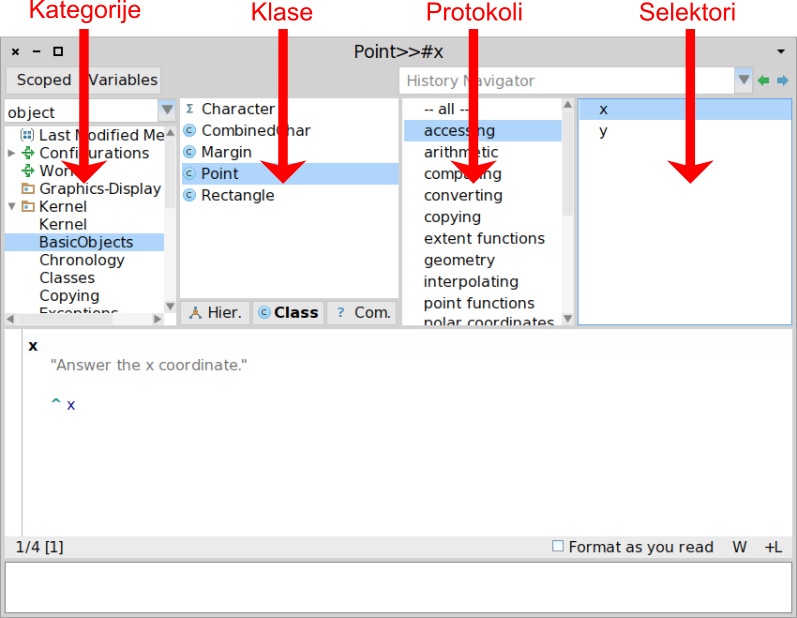
\includegraphics[width=.9\linewidth]{./slike/browser.png}
\end{center}

\subsection{Kreiranje klase}
\label{sec:org49a5bcf}

\begin{center}
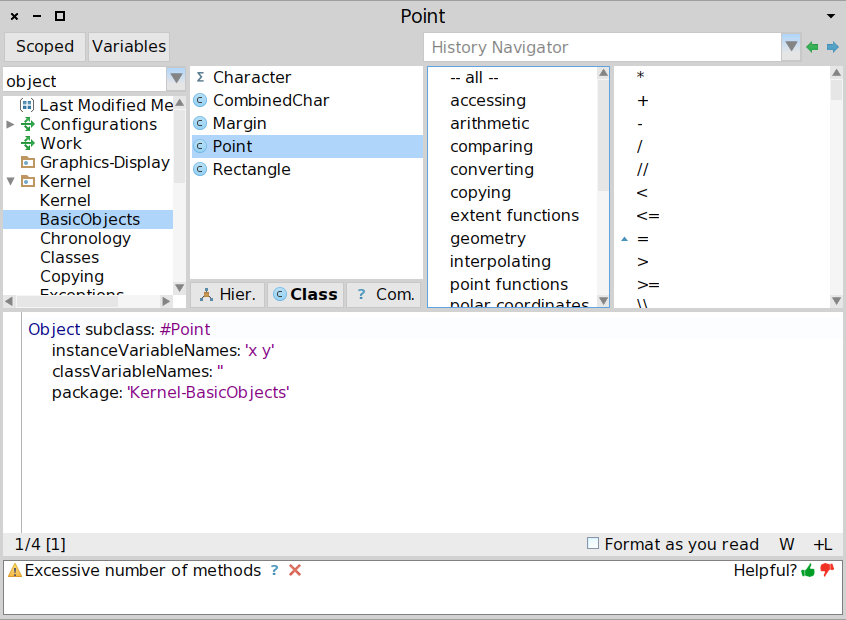
\includegraphics[width=.9\linewidth]{./slike/point_class.png}
\end{center}

\subsection{Kreiranje klase}
\label{sec:orgd32ba50}

Slanje poruke nadklasi

\begin{verbatim}
Object subclass: #Point
  instanceVariableNames: 'x y'
  classVariableNames: ''
  package: 'Kernel-BasicObjects'
\end{verbatim}

\subsection{Definicija metoda}
\label{sec:org1750fae}

\begin{itemize}
\item Metode su javne (\emph{public})
\item Metode su virtualne (tj. pronalaze se u vreme izvršavanja)
\item Podrazumevano vraćaju \texttt{self}
\end{itemize}

\begin{verbatim}
messageSelectorAndArgumentNames
  "comment stating purpose of message"
  
  | temporary variable names |
  statements
\end{verbatim}

\subsection{Primer definicije metode}
\label{sec:orgb755aa5}

\begin{center}
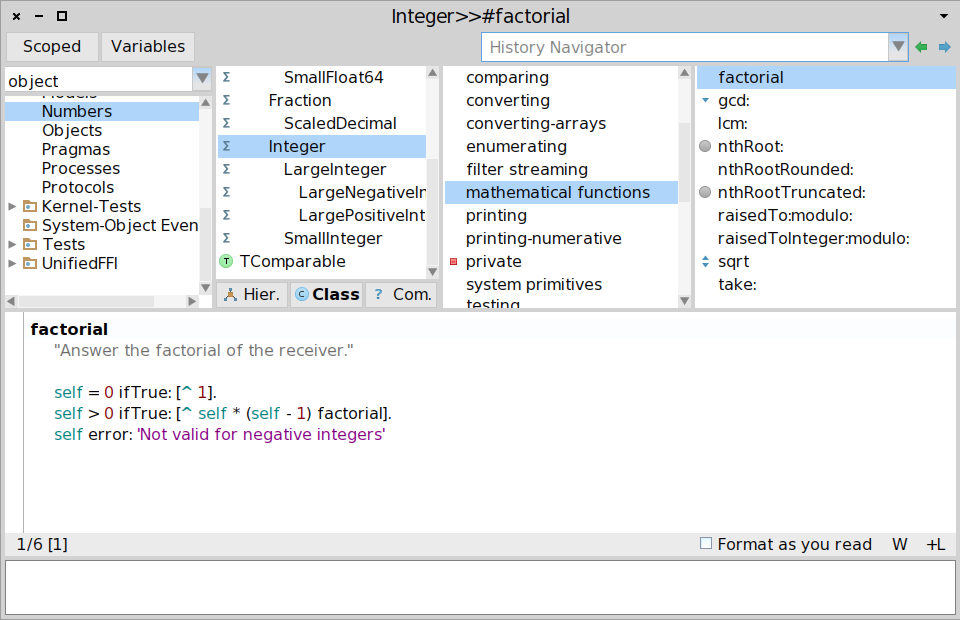
\includegraphics[width=.9\linewidth]{./slike/method_definition.png}
\end{center}

\subsection{Metoda podrazumevano vraća \texttt{self}}
\label{sec:org5a9b5ff}

\begin{verbatim}
Game >> initializePlayers
  self players
  at: 'tileAction'
  put: ( MITileAction director: self )
\end{verbatim}

je ekvivalentno sa:

\begin{verbatim}
Game >> initializePlayers
  self players
  at: 'tileAction'
  put: ( MITileAction director: self ).
  ^ self "<−− optional"
\end{verbatim}

\subsection{Metode klase}
\label{sec:org1be758c}

\begin{center}
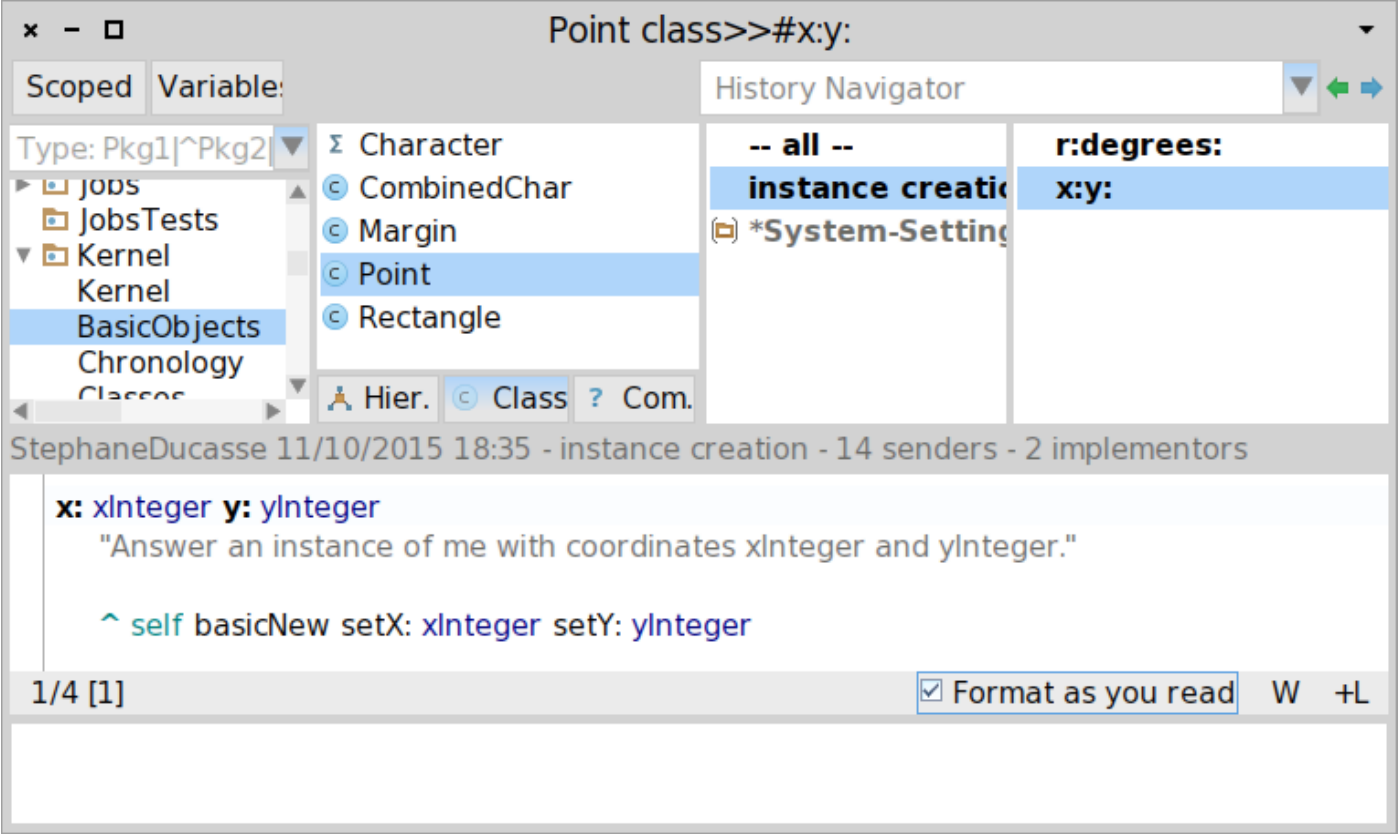
\includegraphics[width=.9\linewidth]{./slike/class_methods.png}
\end{center}

\begin{itemize}
\item Dugme \texttt{Class} služi za pregled i definiciju metoda klase.
\item Metode na nivou klase. Odgovor na poruke koje se šalju klasi.
\end{itemize}

\begin{verbatim}
Point class >> x: xInteger y: yInteger
  "Answer an instance of me with coordinates xInteger and yInteger."

  ^ self basicNew setX: xInteger setY: yInteger
\end{verbatim}
\section{yourself}
\label{sec:org97badb0}
\subsection{Problem}
\label{sec:org8105182}

Dodajemo 2 u skup:

\begin{verbatim}
Set new add: 2
>2
\end{verbatim}

Rezultat izraza je 2 a ne skup!

\subsection{Zašto?}
\label{sec:orgba27597}

\begin{verbatim}
Set>>add: newObject
  "Include newObject as one of the receiver's elements, but
  only if not already present. Answer newObject."
  [...]
  ^ newObject
\end{verbatim}

\begin{itemize}
\item Metod \texttt{add:} vraća argument a ne objekat
\end{itemize}

\begin{verbatim}
Set new add: 2
>2
\end{verbatim}

\subsection{Moguće rešenje}
\label{sec:org5b112a2}

\begin{verbatim}
|s|
s := Set new.
s add: 2.
s
\end{verbatim}

\subsection{Kraće rešenje - \texttt{yourself}}
\label{sec:org8ec7070}

\begin{verbatim}
Object >> yourself
^ self
\end{verbatim}

\begin{verbatim}
Set new
  add: 2;
  yourself
> aSet
\end{verbatim}

\begin{itemize}
\item Poruke \texttt{add:} i \texttt{yourself} se šalju skupu
\item kaskada \texttt{;} vraća objekat koji vraća poruka \texttt{yourself} - u našem slučaju skup.
\end{itemize}

\subsection{Česta greška}
\label{sec:org22940da}

\begin{verbatim}
Counter class >> withValue: anInteger
  self new
  value: anInteger;
  yourself
\end{verbatim}

\begin{itemize}
\item \texttt{Counter withValue: 10} vraća \texttt{Counter} klasu umesto njenu instancu.
\end{itemize}

\subsection{Zašto?}
\label{sec:org909479e}

\begin{verbatim}
Counter class >> withValue: anInteger
  self new
  value: anInteger;
  yourself
\end{verbatim}

je ekvivalentno sa:

\begin{verbatim}
Counter class >> withValue: anInteger
  self new
  value: anInteger;
  yourself.
  ^self
\end{verbatim}

Gde je \texttt{self} prijemnik poruke \texttt{withValue:} tj. klasa \texttt{Counter}.

\subsection{Rešenje}
\label{sec:org35f1e32}

\begin{verbatim}
Counter class >> withValue: anInteger
  ^self new
  value: anInteger;
  yourself
\end{verbatim}

\section{Nasleđivanje i pretraga metoda (\emph{Method Lookup})}
\label{sec:org4eb4e6f}
\subsection{Osnove}
\label{sec:orgca9e877}

Podklasa:
\begin{itemize}
\item Može da doda stanje i ponašanje
\item Može da koristi stanje i ponašanje nadklase
\item Može da izvrši specijalizaciju i redefiniciju ponašanja nadklase
\end{itemize}
\begin{center}
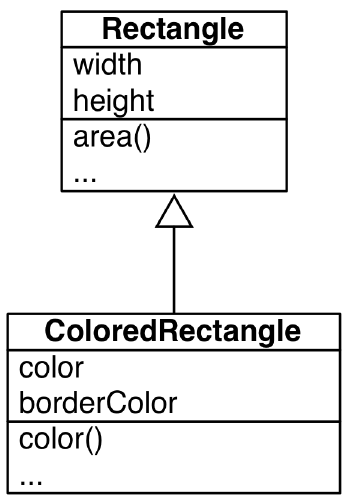
\includegraphics[width=.9\linewidth]{./slike/inheritance.png}
\end{center}

\subsection{Koren hijerarhije nasleđivanja}
\label{sec:org7470c67}

\begin{itemize}
\item Možemo smatrati da je klasa \texttt{Object} korenska klasa svake klase.
\item Postoji i klasa \texttt{ProtoObject} ali je njena upotreba specijalna pa je nećemo
razmatrati.
\end{itemize}
\begin{center}
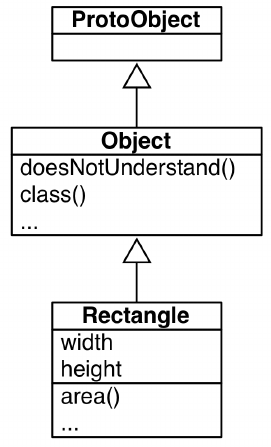
\includegraphics[width=.9\linewidth]{./slike/hierarchy.png}
\end{center}

\subsection{Osnove nasleđivanja}
\label{sec:org40987c8}

Nasleđivanje je:
\begin{itemize}
\item Statičko za stanje (u vreme definisanja klase).
\item Dinamičko za ponašanje (u vreme izvršavanja).
\end{itemize}

\subsection{Nasleđivanje varijabli instanci klasa}
\label{sec:org251c0cf}

\begin{itemize}
\item Dešava se za vreme definicije klase.
\item Izračunava se na osnovu:
\begin{itemize}
\item Varijabli posmatrane klase.
\item Varijabli svih nadklasa.
\end{itemize}
\end{itemize}
\begin{center}
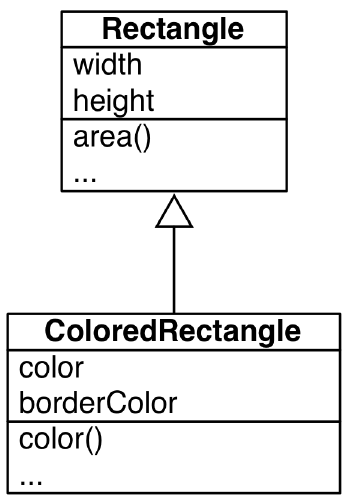
\includegraphics[width=.9\linewidth]{./slike/inheritance.png}
\end{center}

\subsection{Nasleđivanje ponašanja}
\label{sec:org27067e2}

\begin{itemize}
\item Dešava se u vreme izvršavanja
\item Metoda se traži:
\begin{itemize}
\item Počevši od klase objekta prijemnika
\item Zatim u svim nadklasama uz lanac nasleđivanja.
\end{itemize}
\end{itemize}
\begin{center}
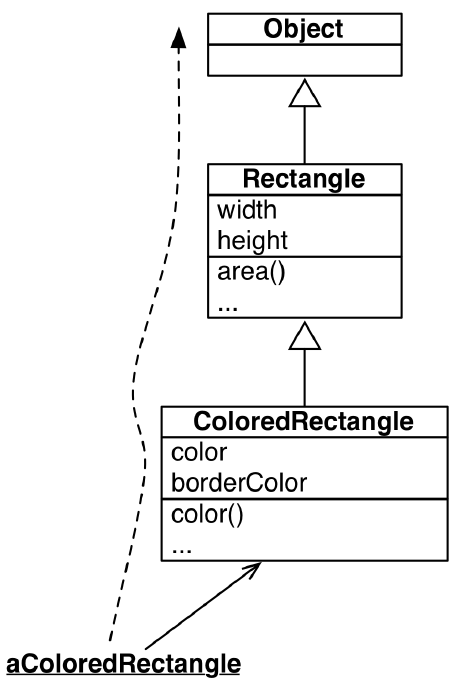
\includegraphics[width=.9\linewidth]{./slike/method_lookup.png}
\end{center}

\subsection{Slanje i obrada poruka}
\label{sec:orgfbb81d3}

Obrada poruke se obavlja u dva koraka:
\begin{enumerate}
\item Pretraga odgovarajuće metode.
\item Izvršavanje metode na objektu prijemniku.
\end{enumerate}
\begin{center}
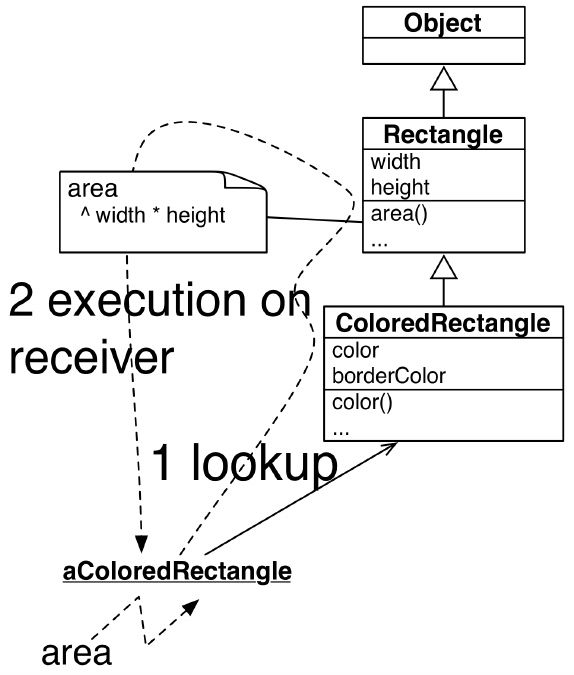
\includegraphics[width=.9\linewidth]{./slike/message_sending.png}
\end{center}

\subsection{Semantika \texttt{self} ključne reči}
\label{sec:org85c16e3}

\begin{itemize}
\item \texttt{self} ključna reč se koristi u implementaciji metoda i \textbf{uvek} predstavlja
objekat prijemnik.
\end{itemize}

\begin{center}
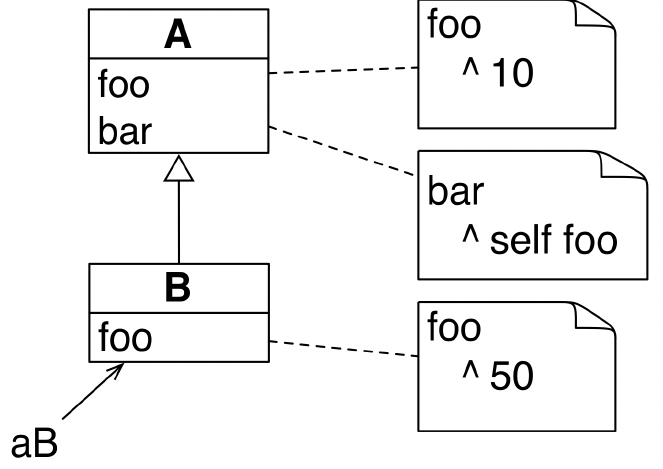
\includegraphics[width=.9\linewidth]{./slike/self_example.png}
\end{center}

\begin{itemize}
\item Šta je rezultat izraza \texttt{A new foo} a šta izraza \texttt{B new foo}?
\item Šta je rezultat izraza \texttt{A new bar} a šta izraza \texttt{B new bar}?
\end{itemize}

\subsection{Semantika \texttt{super} ključne reči}
\label{sec:orga439f62}

\begin{center}
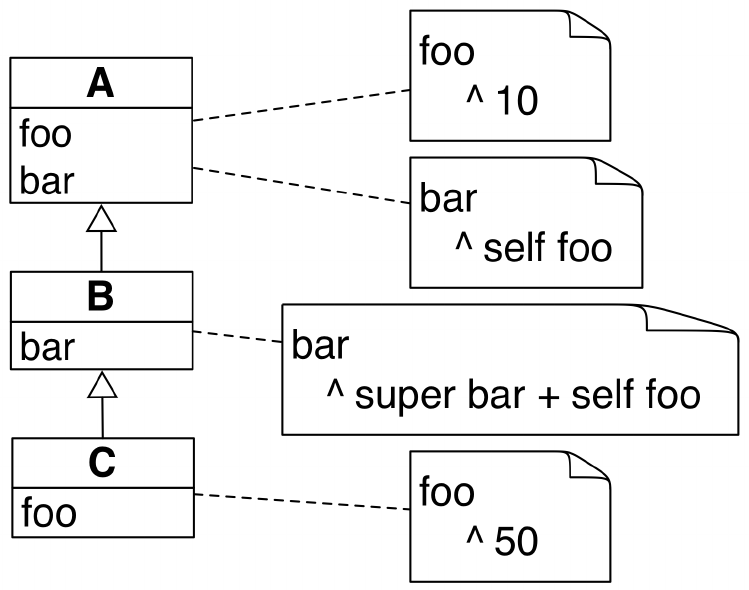
\includegraphics[width=.9\linewidth]{./slike/super_example.png}
\end{center}

\begin{itemize}
\item \texttt{super} predstavlja objekat prijemnik ali pretraga poruka započinje u nadklasi
klase u kojoj se \texttt{super} nalazi.
\item Šta su rezultati izraza \texttt{A new bar}, \texttt{B new bar} i \texttt{C new bar}?
\end{itemize}

\subsection{\texttt{self} se određuje dinamički}
\label{sec:orga0a52ff}

\begin{center}
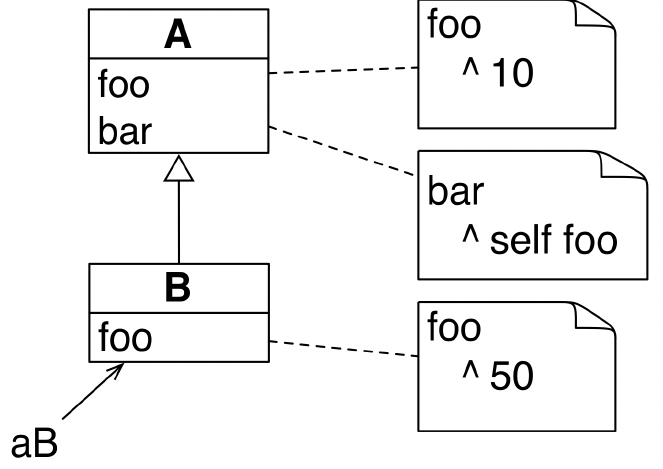
\includegraphics[width=.9\linewidth]{./slike/self_example.png}
\end{center}
U metodi \texttt{A>>bar} kod \texttt{\textasciicircum{}self foo} ne znamo do vremena izvršavanja na koji \texttt{foo}
se poziv odnosi. To zavisi od klase konkretnog objekta prijemnika.

\subsection{\texttt{super} se određuje statički}
\label{sec:org8f20f56}

\begin{center}
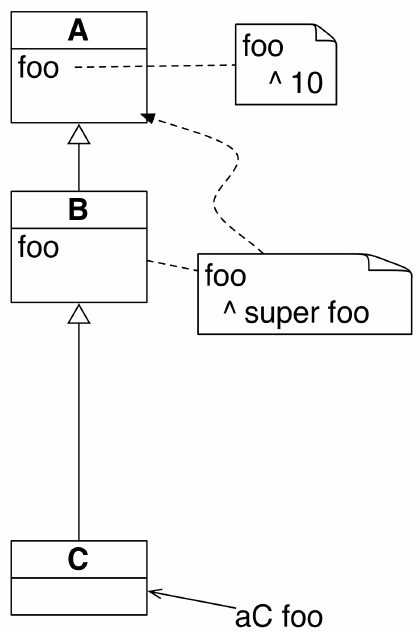
\includegraphics[width=.9\linewidth]{./slike/super_static.png}
\end{center}
\begin{itemize}
\item U vreme kompajliranja znamo da metoda \texttt{B>>foo} referencira \texttt{A>>foo} putem \texttt{super}.
\item Uvek počinjemo pretragu u nadklasi klase koja sadrži metodu koja koristi \texttt{super}.
\end{itemize}

\subsection{Poruke koje nemaju odgovarajuću metodu}
\label{sec:orge18e086}

\begin{itemize}
\item Ukoliko metoda nije pronađena standardnim mehanizmom pretrage, prijemniku se
šalje poruka \texttt{doesNotUnderstand}
\item Podrazumevana implementacija u \texttt{Object} klasi signalizira izuzetak
\texttt{MessageNotUndertood}.
\end{itemize}


\begin{center}
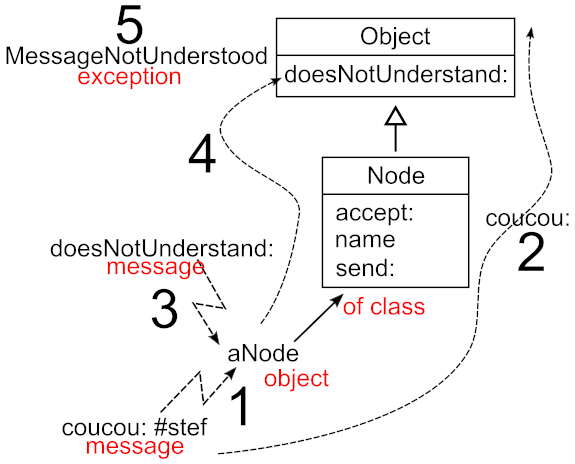
\includegraphics[width=.9\linewidth]{./slike/doesNotUnderstand.png}
\end{center}

\section{Implementacija \texttt{Boolean} tipa}
\label{sec:org5a1882f}
\subsection{Implementacija Boolean tipa}
\label{sec:orgb857ee0}

U Pharo Boolean tip ima odličan dizajn:

\begin{itemize}
\item \texttt{\&, |, not} - \emph{eager}
\item \texttt{or:, and:} - \emph{lazy}
\item \texttt{ifTrue:, ifTrue:ifFalse, ...}
\end{itemize}

\subsection{Za razmišljanje}
\label{sec:org7b915a4}

U svetu gde imate samo dve vrednosti: \texttt{true} i \texttt{false} i razmenu poruka

\begin{itemize}
\item kako implementirati \texttt{not}?
\item kako implementirati \texttt{or}?
\end{itemize}

\subsection{\texttt{not}}
\label{sec:org08db138}

\begin{verbatim}
false not
> true
\end{verbatim}

\begin{verbatim}
true not
> false
\end{verbatim}

\subsection{Bez upotrebe uslova}
\label{sec:org499aed3}

Rešenje ne koristi uslove.

Uslovi bi svakako morali da budu bazirani na Bulovom tipu.

\subsection{Rešenje koristi tri klase}
\label{sec:orga7aa06f}

\begin{itemize}
\item \texttt{Boolean} (apstraktna), \texttt{True} i \texttt{False}
\item \texttt{true} je singlton instanca klase \texttt{True}
\item \texttt{false} je singlton instanca klase \texttt{False}
\end{itemize}

\begin{center}
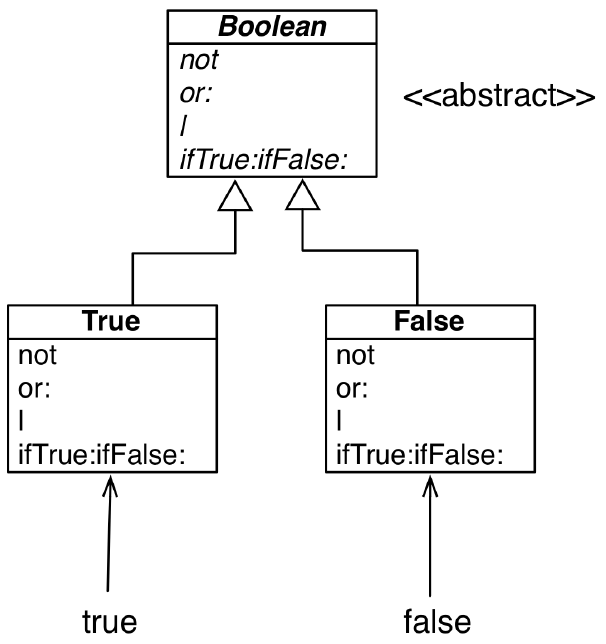
\includegraphics[width=.9\linewidth]{./slike/boolean.png}
\end{center}

\subsection{Kako iskazujemo izbor u OOP?}
\label{sec:orgd70ea5b}

U OOP, izbor iskazujemo:

\begin{itemize}
\item Definisanjem klasa sa kompatibilnim metodama
\item Slanjem poruke instanci takve klase
\end{itemize}

Primer:

\begin{verbatim}
x open
\end{verbatim}

\begin{itemize}
\item \texttt{x} može biti fajl, prozor, alat\ldots{}
\item Metod se selektuje u zavisnosti od klase objekta \texttt{x}
\item U Python-u poznato kao \emph{Duck Typing}
\end{itemize}

\subsection{Implementacija \texttt{not} operacije}
\label{sec:org24bde42}

\begin{verbatim}
False >> not
  "Negation −− answer true since the receiver is false."
  ^ true
\end{verbatim}

\begin{verbatim}
True >> not
  "Negation −− answer false since the receiver is true."
  ^ false
\end{verbatim}

\subsection{Hijerarhija implementacije}
\label{sec:orge0cb7af}

\begin{center}
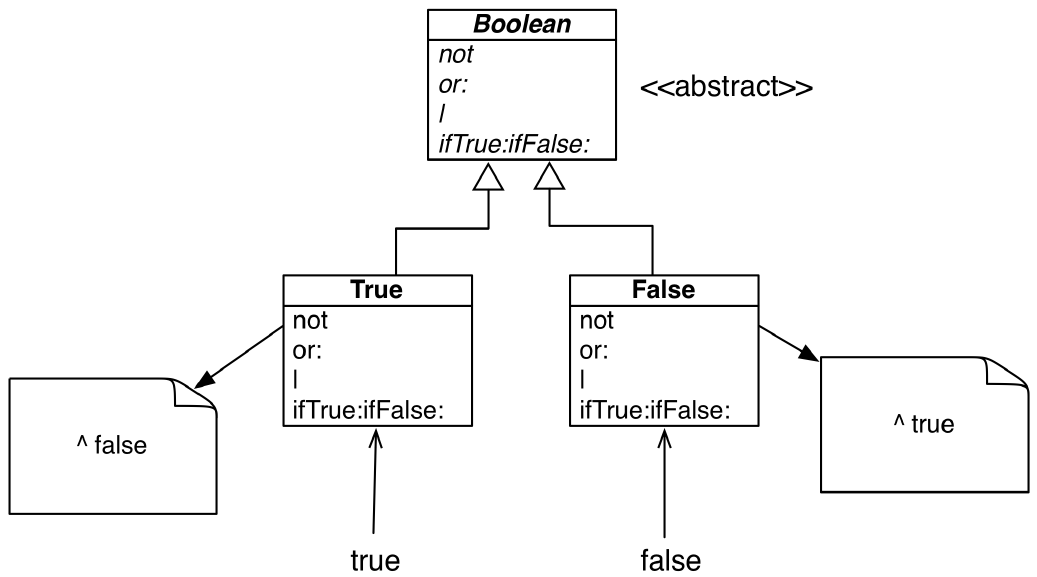
\includegraphics[width=.9\linewidth]{./slike/boolean_not_hierarchy.png}
\end{center}

\subsection{Pretraga poruke (\emph{message lookup}) je izbor prave metode}
\label{sec:org49845f8}

\begin{center}
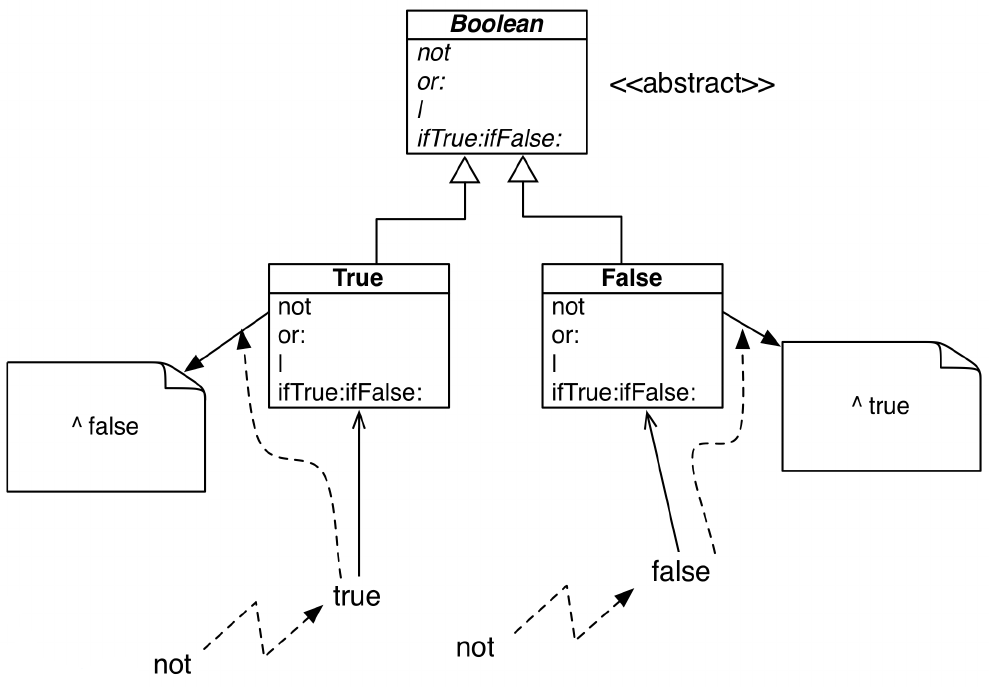
\includegraphics[width=.9\linewidth]{./slike/boolean_not_lookup.png}
\end{center}

\subsection{Implementacija \texttt{Boolean} klase}
\label{sec:org4fb8f66}

\begin{itemize}
\item \texttt{Boolean} je abstraktna klasa
\item Podklase su \texttt{True} i \texttt{False} koje implementiraju:
\begin{itemize}
\item logičke operacije \texttt{\&} i \texttt{not}
\item kontrolne strukture \texttt{and:}, \texttt{or:}, \texttt{ifTrue:}, \texttt{ifFalse:}, \texttt{ifTrue:ifFalse:},
\texttt{ifFalse:ifTrue:}
\end{itemize}
\end{itemize}

\begin{verbatim}
Boolean>>not
  "Abstract method. Negation: Answer true if the receiver is
   false, answer false if the receiver is true."

  self subclassResponsibility
\end{verbatim}

\subsection{Ponašanje \texttt{Or} operacije}
\label{sec:org7a7f6da}

\begin{verbatim}
true | true −> true
true | false −> true
true | anything −> true
\end{verbatim}

\begin{verbatim}
false | true −> true
false | false −> false
false | anything −> anything
\end{verbatim}

\subsection{Implementacija \texttt{Or} operacije u \texttt{Boolean} klasi}
\label{sec:org4904673}

\begin{verbatim}
Boolean >> | aBoolean
  "Abstract method. Evaluating Or: Evaluate the argument.
   Answer true if either the receiver or the argument is true."

  self subclassResponsibility
\end{verbatim}

\subsection{Implementacija \texttt{Or} operacije u klasi \texttt{False}}
\label{sec:org29b1c8e}

\begin{verbatim}
false | true −> true
false | false −> false
false | anything −> anything
\end{verbatim}

\begin{verbatim}
False >> | aBoolean
  "Evaluating Or −− answer with the argument, aBoolean."
  ^aBoolean
\end{verbatim}

\subsection{Implementacija \texttt{Or} operacije u klasi \texttt{True}}
\label{sec:org54796ea}

\begin{verbatim}
true | true −> true
true | false −> true
true | anything −> true
\end{verbatim}

\begin{verbatim}
True >> | aBoolean
  "Evaluating Or −− answer true since the receiver is true."
  ^true
\end{verbatim}

A pošto je prijemnik \texttt{true} možemo uraditi sledeće:

\begin{verbatim}
True >> | aBoolean
  "Evaluating Or −− answer true since the receiver is true."
  ^self
\end{verbatim}

\section{Reference}
\label{sec:org6471919}

\begin{itemize}
\item \href{http://mooc.pharo.org}{Pharo MOOC}
\item \href{http://rmod-pharo-mooc.lille.inria.fr/MOOC/WebPortal/co/pharo.html}{Video lekcije}
\item \href{http://books.pharo.org}{Pharo knjige}
\item \href{https://github.com/pharo-open-documentation/awesome-pharo}{A community-driven collection of awesome Pharo libraries, tools, frameworks and software}
\item \href{http://amber-lang.net/}{Client-side smalltalk - Amber}
\end{itemize}
\end{document}
